% !TeX spellcheck = hu_HU
% !TeX encoding = UTF-8
\chapter{Transformation Tool Contest (TTC)}
\label{sec:ttc}

\newcommand{\ttcyedscale}{0.55}

Az adatok transzformációja az alkalmazások egy széles rétegében központi szerepet tölt be. Ezen alkalmazások erősen függnek az elérhető transzformációs eszközök által nyújtott szolgáltatásokon és azok hatékonyságán. Az alkalmazások fejlesztőinek a számukra legalkalmasabb eszköz kiválasztása nehéz feladat, mivel számos modell- és gráftranszformációs eszköz érhető el manapság. Még a legtapasztaltabb szakemberek is általában egy vagy két eszközt ismernek alaposan, a többiről pedig csak kevés ismeretük van.
Az évente megrendezésre kerülő Transformation Tool Contest (TTC)\footnote{A TTC hivatalos weboldala: \url{https://www.transformation-tool-contest.eu/}} célja, hogy összehasonlítsa a különböző transzformációs eszközök kifejezőerejét, használhatóságát és teljesítményét. 2007 óta minden évben különböző, a valós felhasználások inspirálta feladatokat tesznek közzé, amelyekre bármilyen eszközzel lehet megoldást készíteni. A feladatok a transzformációk felhasználásának széles köréből merítenek ötleteket, többek között:
\begin{itemize}
	\item modell szinkronizáció és egyesítés (merge)
	\item modellek és transzformációk validációja
	\item szemantikus keresés
	\item programok manipulációja és transzformációja
\end{itemize}
Az utóbbi két évben pedig mindig volt egy feladat az \emph{inkrementális nézetkarbantartás} témakörében is. A 2018-as feladatok egyike az LDBC SNB egy egyszerűsített sémája feletti két nézet inkrementális karbantartása volt. A következőkben ezt a feladatot ismertetjük részletesen.

\section{TTC Közösségi háló feladat}

Az TTC 2018 \emph{Közösségi háló} feladatának (Social Media case) egyszerűsített LDBC SNB adatsémáját mutatja be \aref{fig:ttc-schema}.~ábra.
A modellben tehát lehetnek felhasználók (\textsf{User}), akik különböző üzeneteket (\textsf{Submission}) írhatnak (\textsf{submitter} és \textsf{submissions} kapcsolatok): bejegyzéseket (\textsf{Post}) és hozzászólásokat (\textsf{Comment}).
A felhasználók továbbá kedvelhetik (\textsf{likedBy} és \textsf{likes} kapcsolatok) a hozzászólásokat. A felhasználók között lehetőség van barátságok kifejezésére (\textsf{friends} kapcsolatok) is. A hozzászólásokat a felhasználók egy már meglévő üzenethez fűzhetik hozzá (\textsf{comments} és a \textsf{commented} kapcsolatok), tehát a hozzászólásokat reprezentálhatjuk olyan fákkal, ahol egy hozzászólás őse mindig az az üzenet, amelyikre reagáltak az adott hozzászólással. Ekkor belátható, hogy minden ilyen fában pontosan egy bejegyzés lesz, ami a fa gyökere, mivel hozzászólásokat csak meglévő üzenetekhez lehet fűzni. A feladatban a modellek frissítései csak bővítő jellegűek, azaz már meglévő objektumok és kapcsolatok nem törlődnek a modellből, csak újak adódnak hozzá.

Mivel a feladat kiinduló adatmodellje az NMF-fel (\ref{sec:nmf}. szakasz) egyszerűen beolvasható, ezért adott volt a lehetőség a feladatok Naiaddal történő megoldására, mivel a modellek beolvasásához használhattam az NMF-et. Ennek következtében a feladat kiváló lehetőségnek bizonyult
a DAF számítási modell (\ref{sec:differential-dataflow}. szakasz) és 
a Naiad szoftverkönytár (\ref{sec:naiad}. szakasz)
használhatóságának tesztelésére és teljesítménymérésére.

\begin{figure}
	\centering
	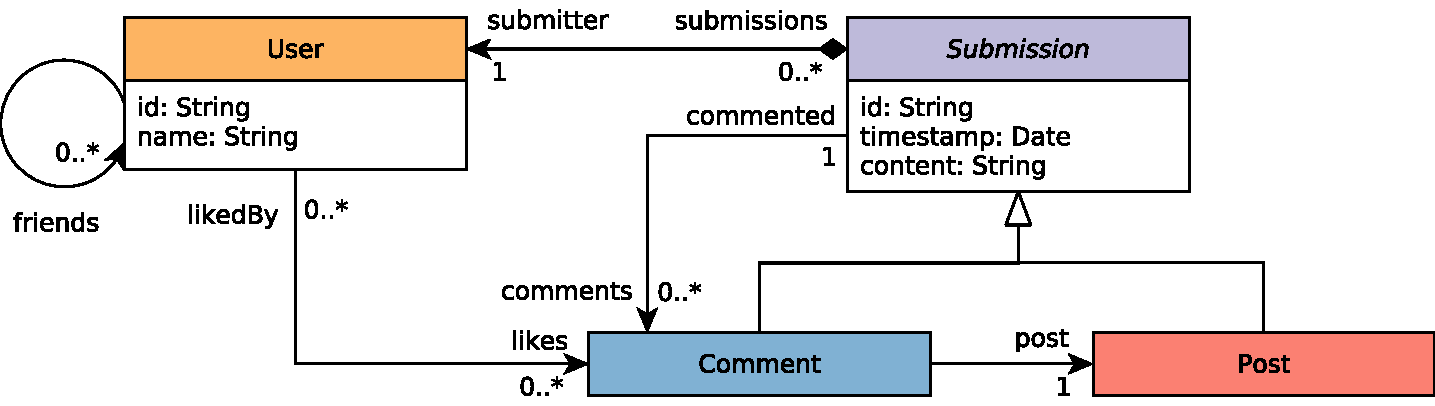
\includegraphics[scale=\ttcyedscale, keepaspectratio]{ttc_schema}	
	\caption{A TTC 2018 Közösségi háló feladatának adatsémája}
	\label{fig:ttc-schema}
\end{figure}

\subsection{A Q1 lekérdezés}

\begin{figure}[ht]
	\centering
	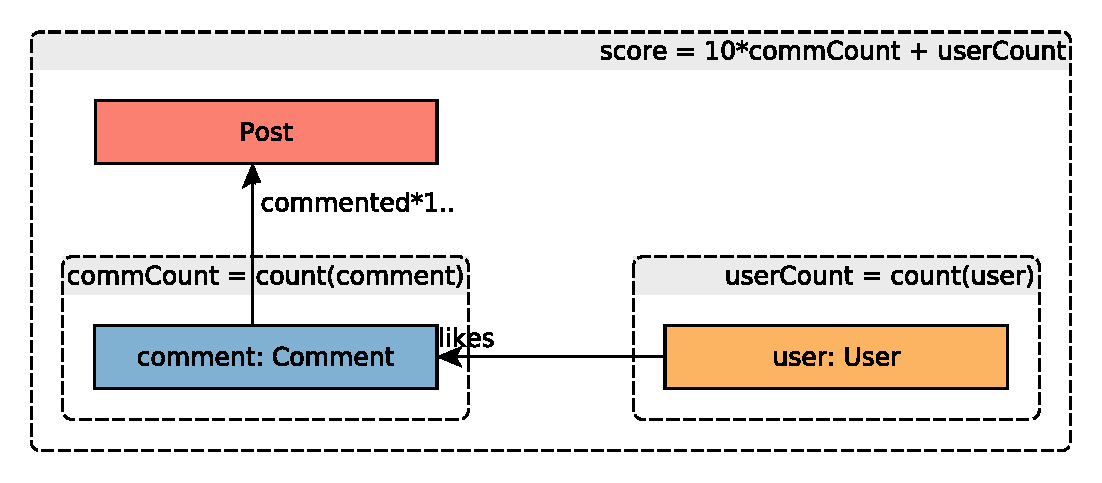
\includegraphics[scale=\ttcyedscale, keepaspectratio]{t1}	
	\caption{A Q1 lekérdezés grafikus ábrázolása}
	\label{fig:ttc-t1}
\end{figure}

Ebben a lekérdezésben a bejegyzéseket pontozzuk a hozzájuk tartozó hozzászólások és kedvelések alapján. A bejegyzések minden hozzájuk tartozó hozzászólás után 10, a bejegyzéshez és hozzászólásokhoz tartozó kedvelések után pedig további 1 pontot kapnak. Egy felhasználó kedvelései több pontot is érhetnek, ha azok különböző üzenetekhez tartoznak. Az így pontozott bejegyzések közül keressük a három legnagyobb pontszámmal rendelkező bejegyzést. Egyenlő pontszámok esetén a korábban létrehozott bejegyzés élvez elsőbbséget. A lekérdezés grafikus szemléltetése látható \aref{fig:ttc-t1}.~ábrán.

A lekérdezés egy konkrét eredményét láthatjuk \aref{fig:ttc-example}.~ábrán. Az ábra felső részén látható a kiindulási állapot \textsf{p1} bejegyzéssel, \textsf{c1} és \textsf{c2} hozzászolásokkal és \textsf{u1}, \textsf{u2}, \textsf{u3} és \textsf{u4} felhasználókkal. A \textsf{p1} bejegyzéshez tartozó pontszám az alábbi részpontszámokból adódik össze:
\begin{itemize}
	\item 20 pont \textsf{c1} és \textsf{c2} hozzászólások miatt
	\item 2 pont a \textsf{c1} hozzászólásra adott kedvelések (\textsf{u2} és \textsf{u3} felhasználó) miatt
	\item 3 pont a \textsf{c2} hozzászólásra adott kedvelések (\textsf{u1}, \textsf{u2} és \textsf{u3} felhasználó) miatt
\end{itemize}
Összesen tehát 25 pontot rendelünk ebben az esetben a \textsf{p1} bejegyzéshez. Az ábra alsó felében a vastagon szedett nyíl jelenti a frissítés által hozzáadott új kedvelést. Ez a kedvelés a \textsf{c2} hozzászóláshoz tartozó kedvelés pontjait növeli meg 3-ról 4-re, így a \textsf{p1} bejegyzés pontszáma 26-ra módosul.

\subsection{A Q2 lekérdezés}

\begin{figure}[ht]
	\centering
	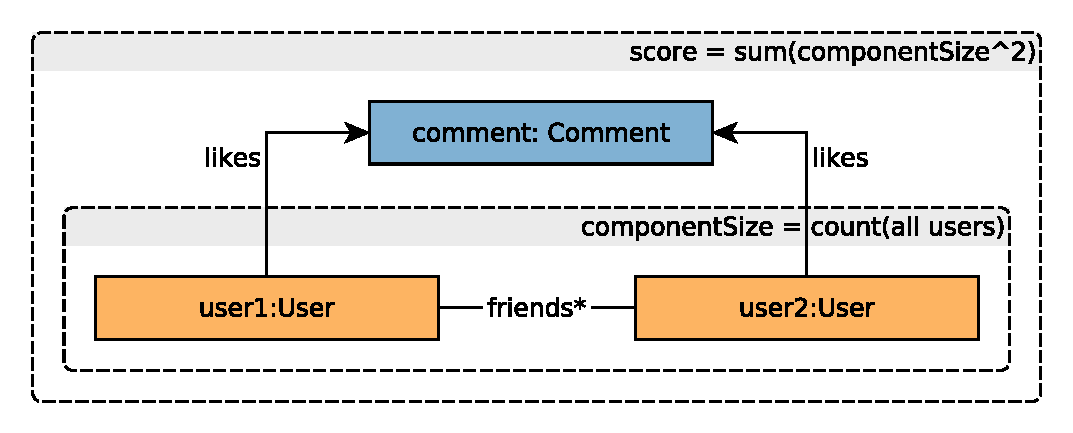
\includegraphics[scale=\ttcyedscale, keepaspectratio]{t2}	
	\caption{A Q2 lekérdezés grafikus ábrázolása}
	\label{fig:ttc-t2}
\end{figure}

Ebben a lekérdezésben azokat a hozzászólásokat keressük, amelyek a felhasználók legnagyobb csoportjai által kedveltek. A felhasználó csoportokat a barátság kapcsolaton keresztül azonosítjuk: egy adott hozzászólást kedvelő felhasználók közül egy csoportba tartoznak azok a felhasználók, akik a barátság kapcsolatokon keresztül összefüggő komponenseket (strongly connected components, SCC) alkotnak.
Tehát egy olyan gráfban keresünk összefüggő komponenseket, ahol a hozzászólást kedvelő felhasználók a csúcsok, és a közöttük lévő barátság kapcsolatok pedig az élek. Az összefüggő komponensek azonosítása után összegezzük a komponensek méretének négyzetösszegét. A lekérdezés grafikus szemléltetése látható \aref{fig:ttc-t2}.~ábrán.

\Aref{fig:ttc-example}.~ábrán szintén láthatjuk a lekérdezés egy konkrét eredményét. A \textsf{p1} bejegyzés pontszáma a következő részpontszámokból adódik össze:
\begin{itemize}
	\item $2 \times 2 = 4$ pont a \textsf{c1} hozzászólást kedvelő felhasználók miatt, mivel ők egy 2 elemű komponenst alkotnak
	\item $2 \times 2 + 1 \times 1 = 5$ pont a \textsf{c2} hozzászólást kedvelő felhasználók miatt, mivel egy 1 elemű (\textsf{u1}) és egy 2 elemű (\textsf{u3} és \textsf{u4}) komponenst alkotnak
\end{itemize}
Összesen tehát a \textsf{p1} bejegyzéshez 9 pontot rendelünk. Az ábra alsó felében, a frissítés után látható, hogy a \textsf{c2} hozzászólást kedvelő felhasználók immár egy 4 elemű komponenst alkotnak, tehát a \textsf{c2}-höz tartozó részpontszám 16-ra ($4 \times 4$) változik, így a \textsf{p1} bejegyzés pontszáma pedig 20 pontra változik.

\begin{figure}
	\centering
	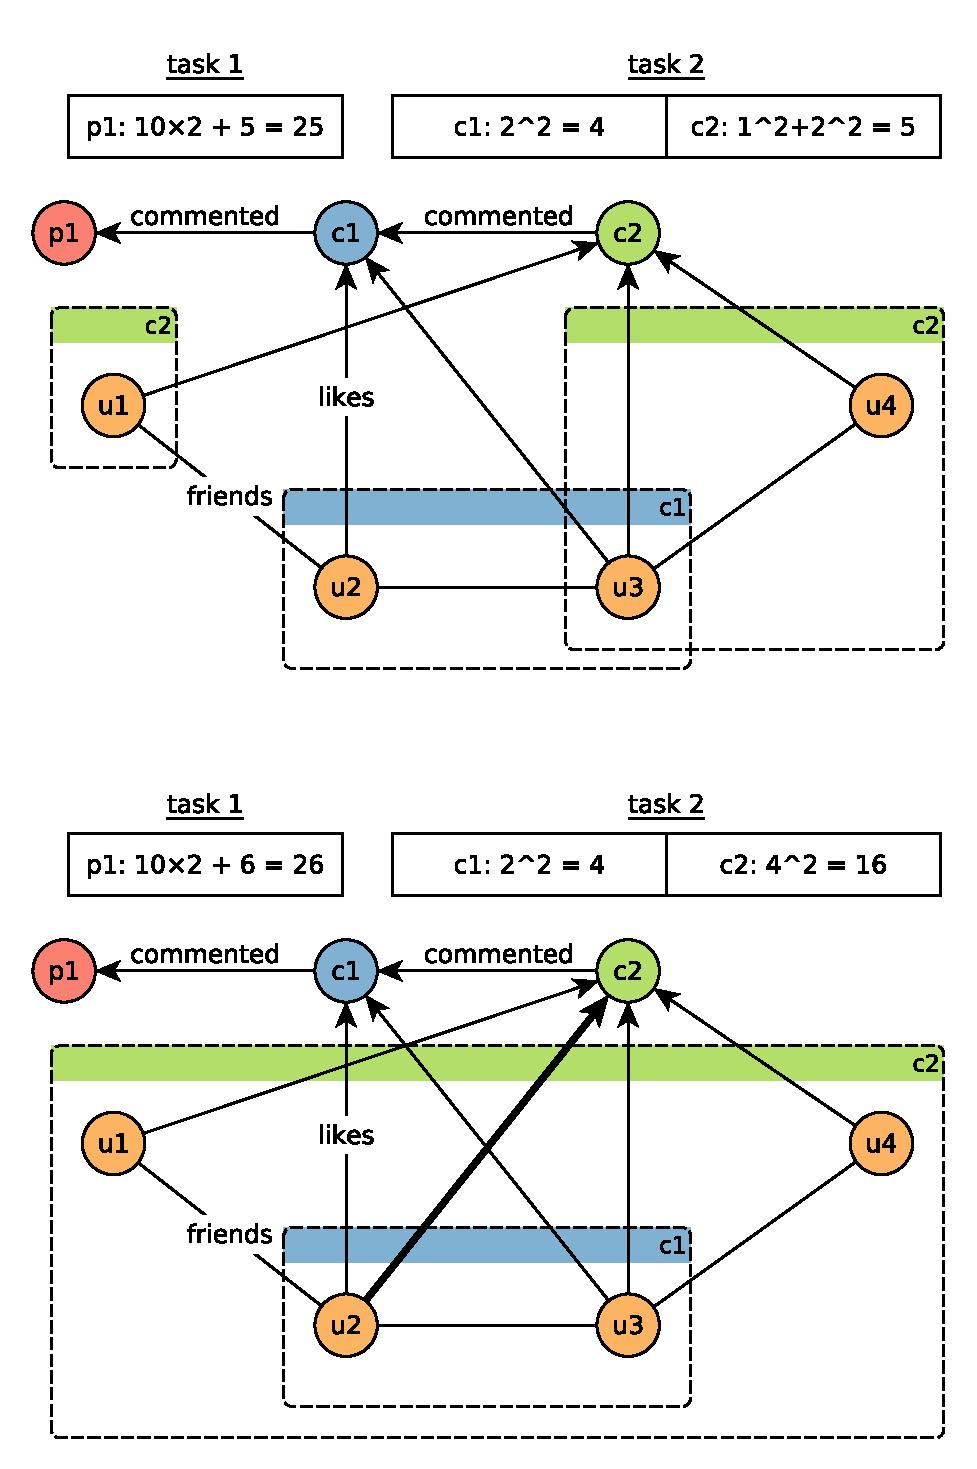
\includegraphics[scale=\ttcyedscale, keepaspectratio]{ttc-example}	
	\caption{A lekérdezések eredményének grafikus ábrázolása. A második modellben a vastag él az újonnan hozzáadott élet jelöli.}
	\label{fig:ttc-example}
\end{figure}

\subsection{Megoldás ismertetése}

A megoldás során a Naiad könyvtárban rendelkezésre álló DAF keretrendszert használtam. A keretrendszer a relációs lekérdezőnyelvekben használatos operátorok (\keyword{SELECT}, \keyword{JOIN}, \keyword{DISTINCT}, \keyword{COUNT}, \keyword{SUM} stb.) DAF alapú megvalósításán túl további operátorokat is definiál. A megoldásaim három olyan operátort használnak, amelyek túlmutatnak vagy nem megszokottak a relációs lekérdezőnyelvek világán:
\begin{itemize}
	\item \uline{\texttt{FixedPoint}:} A \texttt{FixedPoint} operátor használatával definiálhatjuk a DAF-ban említett ciklusokat. A ciklusok létrehozásakor meg kell adni azt a DAF-ot, amit a ciklus belsejében szeretnénk végrehajtani, valamint a DAF bemenetének számító adatforrást. Az operátor nevével összhangban egy iterációban addig hajtja végre a beágyazott DAF-ot, amíg annak kimenete két iteráció között megváltozik. A beágyazott DAF bemenetének típusa természetesen meg kell egyezzen a kimenetének típusával, így lehet ciklusként végrehajtani. Az operátor által létrehozott ciklust az úgynevezett \texttt{LoopContext} objektum azonosítja. Az operátor használatára a Q1 esetében a bejegyzésekhez tartozó hozzászólások (tranzitív lezártak) keresésekor, a Q2 esetében pedig az összefüggő komponensek keresésekor volt szükség.
	\item \uline{\texttt{EnterLoop}:} A \texttt{FixedPoint} operátor alapértelmezetten csak egy adatforrást támogat, azonban lehetőség van a ciklusokon belül több adatforrást is használni az \texttt{EnterLoop} operátor használatával. Bemenete egy adatforrást reprezentáló objektum és egy \texttt{LoopContext} objektum, kimenete pedig egy olyan adatforrást reprezentáló objektum, ami már használható a beágyazott DAF-ban is. Használatát a \texttt{FixedLoop} használatának szükségessége indokolta.
	\item \uline{\texttt{CoGroupBy}:} A Naiad által nyújtott DAF keretrendszer nem definiál külső illesztéseket végrehajtó operátorokat, azonban a \texttt{CoGroupBy} operátor nagyon hasonló szemantikával rendelkezik, használatával megvalósíthatóak a külső illesztések. Az operátor bemenete két adatforrás és a hozzájuk tartozó kulcsderiváló függvények. Az operátor a kulcsok szerint csoportosítja a két adatforrásból érkező adatrekordokat, így \textsf{<key, list1, list2>} hármasokat állít elő belőlük, ahol a \textsf{key} a közös kulcs, \textsf{list1} és \textsf{list2} pedig rendre az első és a második adatforrásból a  kulcshoz tartozó adatrekordok listája. A \texttt{CoGroupBy} operátort a hozzászólásokhoz tartozó kedvelések megszámolására használtam.
\end{itemize}
A Q1 lekérdezés differenciális adatfolyamának szemléltetése \aref{fig:q1-ddffig}.~ábrán látható, amelyeken megfigyelhető a \texttt{FixedPoint} és a \texttt{EnterLoop} operátorok kapcsolata.